\documentclass[conference]{IEEEtran}

\usepackage{cite}
\usepackage{amsmath,amssymb,amsfonts}
\usepackage{algorithmic}
\usepackage{graphicx}
\usepackage{textcomp}
\usepackage{xcolor}
\def\BibTeX{{\rm B\kern-.05em{\sc i\kern-.025em b}\kern-.08em
    T\kern-.1667em\lower.7ex\hbox{E}\kern-.125emX}}


\usepackage[utf8]{inputenc}
\usepackage{url}
\usepackage{listings}
\usepackage{hyperref}
\lstset{basicstyle=\ttfamily}
\usepackage{caption}

\lstdefinestyle{mypython}{
    language=Python,              % Language to be used
    backgroundcolor=\color{white}, % Background color
    basicstyle=\ttfamily\small,   % Font size and type
    breaklines=true,               % Automatically break long lines
    captionpos=b,                  % Caption position (bottom)
    numbers=left,                  % Line numbers on the left
    numberstyle=\tiny\color{gray}, % Style for line numbers
    frame=single,                  % Frame around the code
    escapeinside={(*@}{@*)},       % For adding LaTeX inside the code
}

\setlength{\columnsep}{20pt}  % Adjust the space between columns




\title{Lung Sound Detection and Classification}


\author{
\IEEEauthorblockN{Karthik Venkat Malavathula}
\IEEEauthorblockA{
\textit{Embedded Systems Workshop} \\
\textit{IIIT Hyderabad} \\
Hyderabad, India \\
karthikvenkat.m@research.iiit.ac.in
}
\and
\IEEEauthorblockN{Anurag Peddi}
\IEEEauthorblockA{
\textit{Embedded Systems Workshop} \\
\textit{IIIT Hyderabad} \\
Hyderabad, India \\
anurag.peddi@students.iiit.ac.in
}
\\[0.5cm] % Line break with vertical spacing
\IEEEauthorblockN{Adithya Addepalli Casichetty}
\IEEEauthorblockA{
\textit{Embedded Systems Workshop} \\
\textit{IIIT Hyderabad} \\
Hyderabad, India \\
adithya.addepalli@students.iiit.ac.in
}
\and
\IEEEauthorblockN{Aryanil Panja}
\IEEEauthorblockA{
\textit{Embedded Systems Workshop} \\
\textit{IIIT Hyderabad} \\
Hyderabad, India \\
aryanil.panja@research.iiit.ac.in
}
}


\begin{document}

\maketitle


\begin{abstract}
In this project, we aim to present a comprehensive approach to lung sound detection and classification using various filtering and machine-learning techniques.
% SECTIONS:
% \begin{itemize}
%     \item Introduction
%     \item flow of Execution
%     \item Recording Data
%     \begin{itemize}
%         \item Methods Used (phone)
%         \item Spectrography
%         \item Noise Conditions
%         \begin{itemize}
%             \item Low Noise
%             \item Medium Noise
%             \item High Noise
%         \end{itemize}
%     \end{itemize}
%     \item Filtering
%     \begin{itemize}
%         \item Band-pass
%         \item blah blah filter ( i have no idea)
%         \item Spectral Gating
%         \item Master Algorithm
%     \end{itemize}
%     \item Linking 
%     \begin{itemize}
%         \item Python
%     \end{itemize}
%     \item Model
%     \begin{itemize}
%         \item SVM
%         \item CNN
%     \end{itemize}
%     \item hardware
%     \begin{itemize}
%         \item 3-D modeling
%         \item Tapes 
%     \end{itemize}
%     \item 
% \end{itemize}
\end{abstract}

\begin{IEEEkeywords}
band-pass, wavelet transform, spectral gating, SVM, CNN, INMP441, Mel Spectrogram
\end{IEEEkeywords}

\section*{Introduction}
Accurate detection and analysis of lung sounds are crucial in
biomedical signal processing. This work focuses on developing
a pipeline for real-time sound analysis involving noise filtering
using a band-pass filter, wavelet decomposition, and spectral gating. It further specifies models to neatly classify data based on the recording.

\section{Recording Data}
The first step in our project was to record heart/lung sounds using the INMP441. This we achieved through a combination of code and hardware.

\subsection{Challenges Faced}

During the course of this project, we encountered several significant challenges. One major issue was the poor quality of the initial recordings, necessitating multiple attempts to obtain satisfactory samples. Additionally, we experienced indecision regarding the best recording method, as we explored various options such as using a phone, laptop, or other recording devices. Our limited familiarity with sound technology further complicated the process, requiring us to learn essential terminology, including concepts like "Mel spectrogram," which were crucial for analyzing the recorded data effectively.

\subsection{Process and Findings (Karthik)}

To capture the sound of a heartbeat, I used my phone to record in three distinct environments, each presenting varying levels of ambient interference. The first recording, characterized by low interference, was made in a completely silent environment in our room, serving as a clear and unobstructed baseline for comparison. The second recording, representing medium interference, was taken at night when the gentle sounds of crickets provided a constant but subtle background noise, ideal for testing moderate levels of interference. The third recording, indicative of high interference, occurred in the presence of a loud spinning fan and external noise from an amphitheater, introducing significant background disruptions.

In addition to recording the audio, I created before-and-after spectrograms for the WAV files using the Sonic Recorder application. These spectrograms visually represented the frequency spectrum of the audio recordings, enabling a detailed analysis of how the varying levels of interference affected the clarity of the heartbeat sounds. This process not only highlighted the differences in sound quality across the three environments but also provided valuable insights into the challenges of capturing clear audio in noisy conditions. The spectrograms served as a critical tool for understanding the impact of ambient noise and informed our approach to refining the recording process.


\subsection{Mel Spectrogram}

\begin{figure}
    \centering
    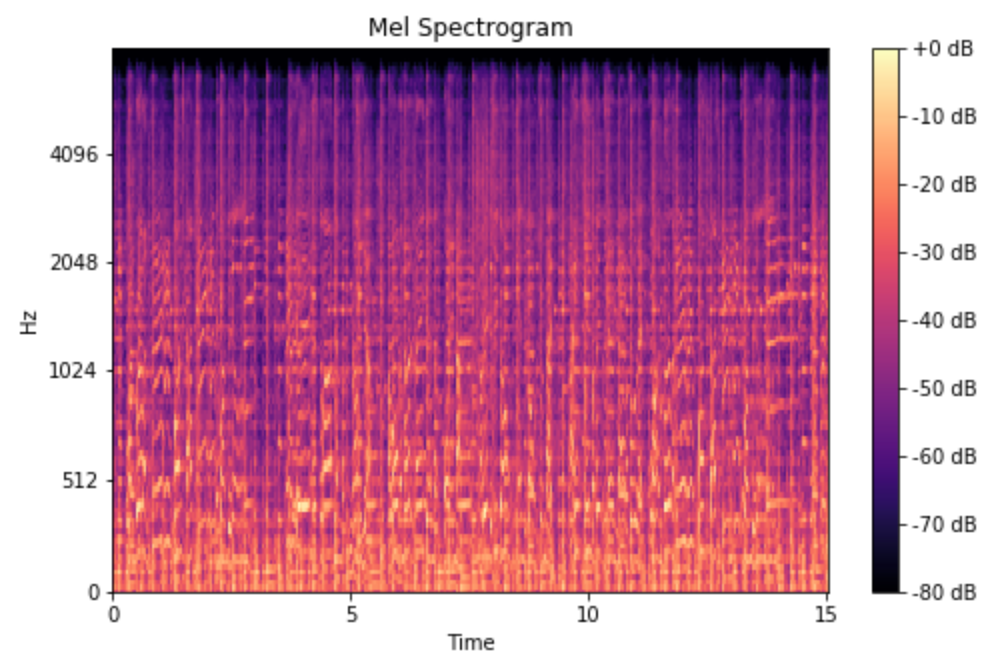
\includegraphics[width=0.5\textwidth]{Images/Melspectrogram.png}
    \caption{Example of a Mel Spectrogram}
    \label{fig:mel_spectrogram}
\end{figure}

A Mel spectrogram is a visual representation of the spectrum of frequencies in an audio signal over time, transformed into the Mel scale. The Mel scale is designed to mimic the way humans perceive sound, focusing on the fact that our ears are more sensitive to lower frequencies than higher ones. To create a Mel spectrogram, the audio signal is first divided into small time segments (frames) using a process called Short-Time Fourier Transform (STFT). The resulting frequency data is then mapped onto the Mel scale, compressing the higher frequencies to better match human auditory perception.

In this project, Mel spectrograms were invaluable for analyzing the quality of heartbeat recordings. They allowed us to visualize how ambient noise influenced the clarity of the heartbeat across different environments. The spectrograms helped identify which frequencies were most affected by noise and how interference altered the distinct frequency patterns associated with the heartbeat.

\subsection{Noise Cases (Karthik)}

\begin{figure}
    \centering
    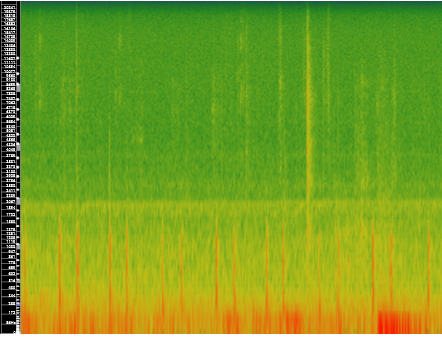
\includegraphics[width=0.4\textwidth]{Images/lownoise.png}
    \caption{Low Interference Mel Spectrogram}
    \label{fig:mel_spectrogram}
\end{figure}

\textbf{Low Interference:}  
In the low-interference case, the recording was made in a silent environment, free from ambient noise. The resulting Mel spectrogram showed clean, distinct frequency patterns corresponding to the heartbeat, with minimal background noise. This recording served as a baseline for comparison, highlighting what a clear heartbeat should look like in an ideal setting.

\begin{figure}
    \centering
    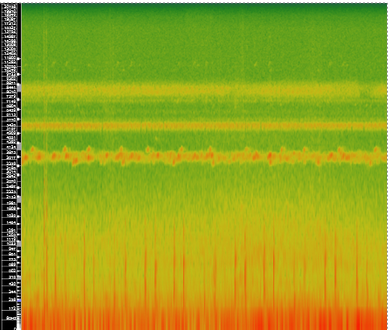
\includegraphics[width=0.4\textwidth]{Images/midnoise.png}
    \caption{Medium Interference Mel Spectrogram}
    \label{fig:mel_spectrogram}
\end{figure}

\textbf{Medium Interference:}  
The medium-interference recording occurred at night, accompanied by the soft, constant sound of crickets. The Mel spectrogram displayed the heartbeat frequencies clearly but with a subtle background layer representing the crickets’ chirping. This environment provided a useful middle ground, demonstrating how a moderate level of constant noise influences audio clarity without overwhelming the main signal.

\begin{figure}
    \centering
    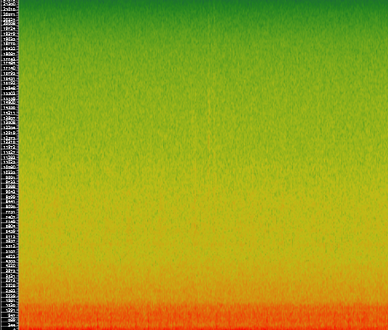
\includegraphics[width=0.4\textwidth]{Images/loudnoise.png}
    \caption{High Interference Mel Spectrogram}
    \label{fig:mel_spectrogram}
\end{figure}

\textbf{High Interference:}  
In the high-interference scenario, the recording was done in the presence of a loud spinning fan and external noise from an amphitheater. The Mel spectrogram for this case showed a significant amount of background noise, with the heartbeat frequencies partially obscured by broader frequency bands. This example underscored the challenges of capturing clear audio in noisy conditions, as the strong interference made it more difficult to isolate the heartbeat signal.

Together, these noise cases illustrated the varying effects of ambient interference on audio quality, emphasizing the importance of minimizing noise in critical sound recording applications such as heartbeat monitoring.


\subsection{Initial Recording Features (Anurag)}
The ESP32 was programmed to record audio using the INMP441 microphone. The initial developed recording code included the following features:
\begin{itemize}
    \item Records sound and creates a WAV file stored in the ESP32’s memory.
    \item Adjustable sample rate to control recording quality.
    \item Configurable sample bits to manage audio fidelity.
    \item Customizable recording duration for varied application requirements.
\end{itemize}

\begin{figure}[h]
    \centering
    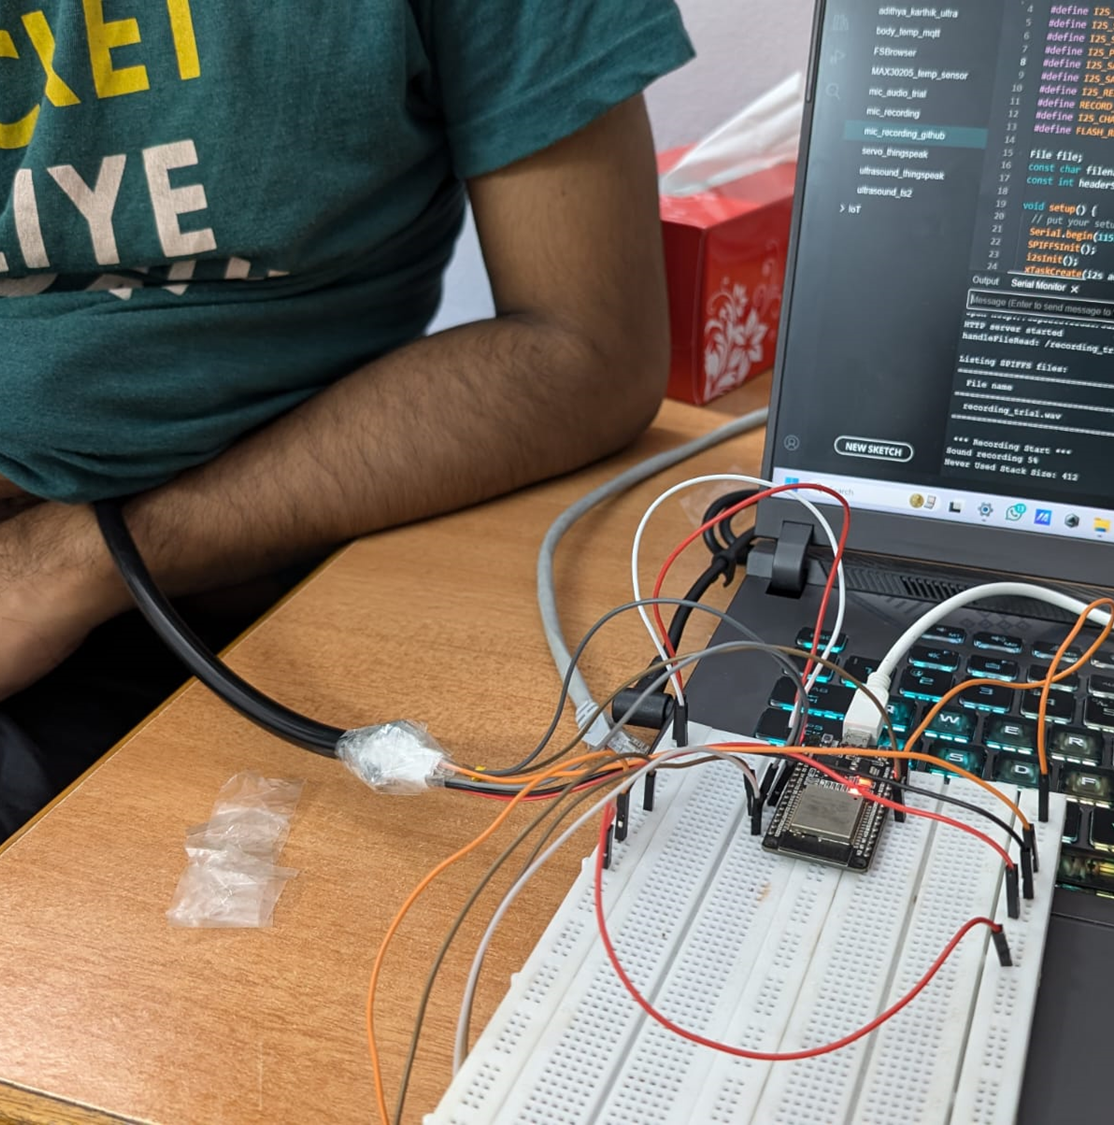
\includegraphics[width=0.5\linewidth]{Images/first_trial.png}
    \caption{First Recording Trial}
    \label{fig:enter-label}
\end{figure}

\subsection{Initial Trials}
The first attempts at recording heartbeat and lung sounds were conducted using the stethoscope. Recordings made through direct skin contact yielded better results compared to over-clothing placement. However, the captured audio was noisy, with no discernible heartbeats or lung sounds, even after applying noise filtering. In contrast, sounds recorded directly from a computer were clearer and exhibited distinct heartbeats post-filtering.

\begin{figure}[h]
    \centering
    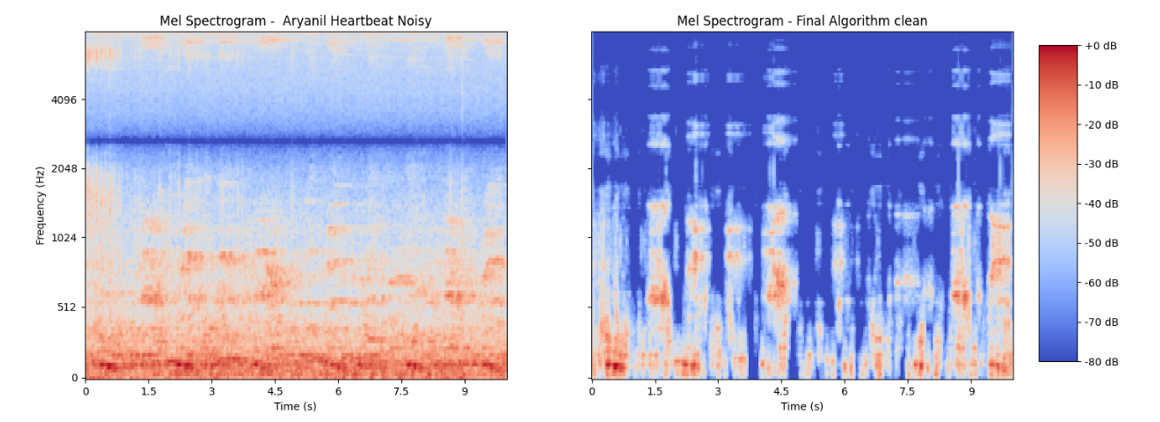
\includegraphics[width=1\linewidth]{Images/trial_spectrogram.png}
    \caption{Mel Spectrogram of the first trial before and after filtering}
    \label{fig:enter-label}
\end{figure}

\begin{figure}[h]
    \centering
    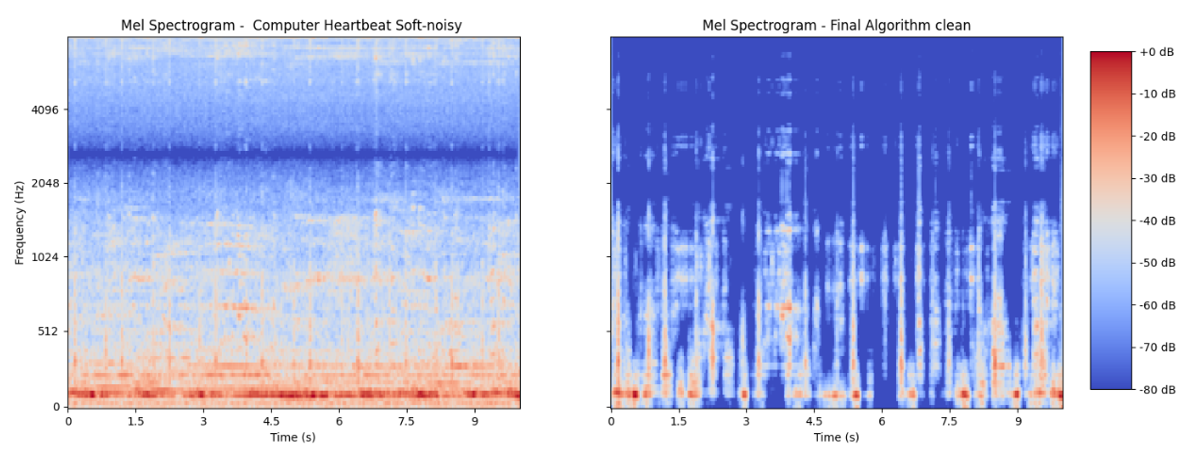
\includegraphics[width=1\linewidth]{Images/computer_spectrogram.png}
    \caption{Mel Spectrogram of sound recorded from the computer before and after filtering}
    \label{fig:enter-label}
\end{figure}

\subsection{Updated Recording Features (Anurag)}
Instead of recording and saving a WAV file as we did initially, this time we directly saved the recorded input as a RAW file, preserving data quality. This included the following features:
\begin{itemize}
    \item Records sound and creates a RAW file stored in the ESP32’s memory.
    \item Adjustable sample rate to control recording quality.
    \item Configurable sample bits to manage audio fidelity.
    \item Customizable recording duration for varied application requirements.
\end{itemize}



\section{Hardware}

\subsection{Hardware Setup}
Initially, to accommodate the sensors and ESP32, an expanded hardware setup was created by connecting two breadboards. The ESP32 and sensors were securely positioned, and modifications were made to a stethoscope to improve sound capture. Medical tape was used to secure wiring, while cello tape helped reduce noise.

However, the breadboard caused a lot of electrical interference in the mic, leading to noisy recordings. Also, the tapes used were not sufficient to drown out external noise.

\begin{figure}[h!]
    \centering
    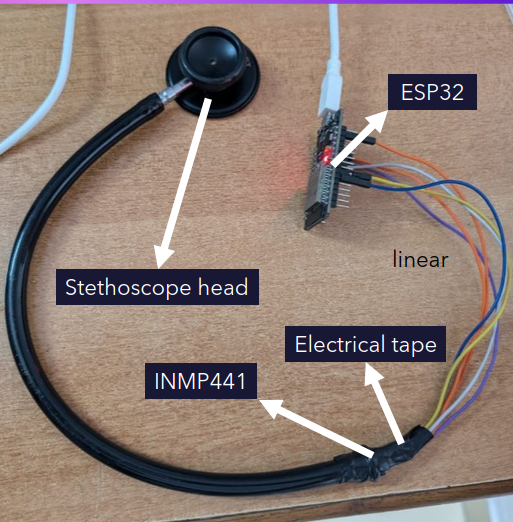
\includegraphics[width=0.4\textwidth]{Images/setup.png}
    \caption{Final Hardware Setup}
\end{figure}

\subsection{Final Hardware Setup}

The system uses four primary components. The \textbf{stethoscope head} is utilized to capture acoustic signals directly from the body. It is specifically designed to detect low-frequency sounds, making it highly effective for medical auscultation. The \textbf{INMP441 microphone sensor} is a digital I\textsuperscript{2}S microphone known for its high signal-to-noise ratio (SNR) and low power consumption. It ensures accurate sound capture without the need for analog signal processing. The \textbf{ESP32 microcontroller} acts as the central processing unit, offering Wi-Fi and Bluetooth capabilities for wireless data transmission. Finally, \textbf{electrical tape} is used to secure the connections between the stethoscope head and the microphone, providing a flexible and adjustable solution.

\subsection{Features and Advantages}

One of the key advantages of this setup is the use of a stethoscope head for direct sound capture, which filters out many ambient noises and ensures the precise detection of lung sounds. Unlike generic microphones, the stethoscope head is optimized for body sound detection, making it ideal for this application.
         
The INMP441 microphone sensor, with its digital interface, eliminates the need for analog signal processing, reducing the risk of noise from analog circuitry. This provides a clearer and more accurate representation of lung sounds compared to traditional analog microphones. The ESP32 microcontroller enhances the system's versatility by providing onboard data processing and multiple connectivity options. Unlike simpler microcontrollers, the ESP32 allows real-time data transmission via Wi-Fi or Bluetooth, which is essential for remote monitoring applications. 

\subsection{3D Printing a tube covering (Karthik, Anurag)}
      
\begin{figure}
    \centering
    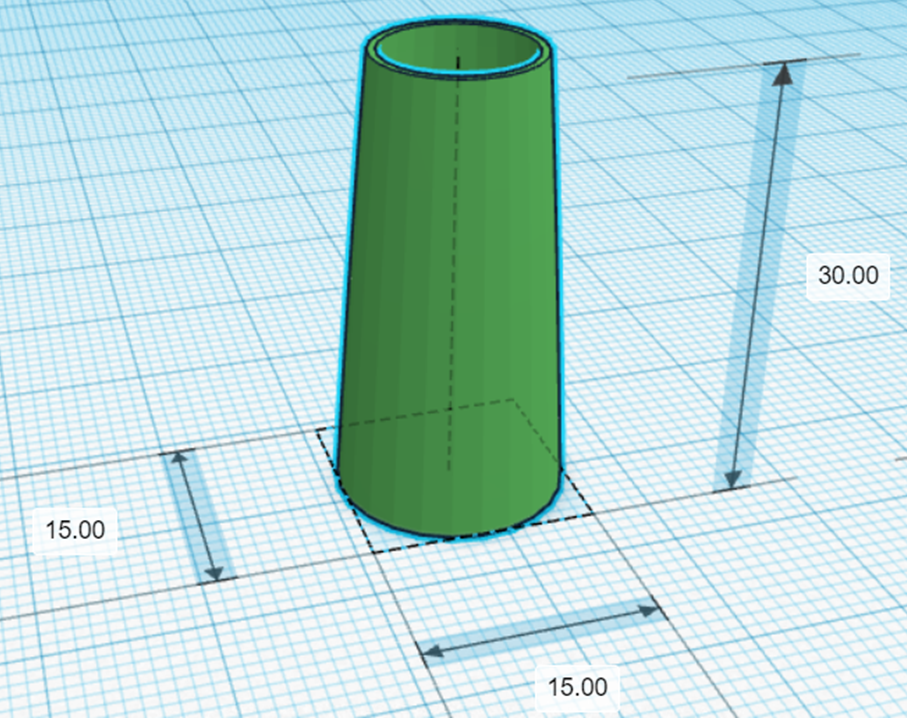
\includegraphics[width=0.5\linewidth]{Images/3dprint1.png}
    \caption{One of the 3D printing models we considered}
    \label{fig:enter-label}
\end{figure}

We briefly considered using 3D printing to connect connect the stethoscope head and the microphone sensor. We created iterations of models to use, and some of the most promising ones were shown above. However, we collectively decided not to opt for this decision. Instead of using 3D printing to connect the stethoscope head and the microphone sensor, electrical tape was chosen due to its flexibility and adaptability. Electrical tape allows for easy adjustments to the positioning and alignment of the components, which would be difficult with a rigid 3D-printed connector. Additionally, it is a cost-effective and time-efficient solution, especially during the prototyping phase. Furthermore, electrical tape provides good noise isolation by dampening mechanical vibrations, which might not be achieved with a rigid 3D-printed part.




\section{Data Transmission (Anurag)}
After recording the sound, we had to pass it to Python for further processing. We tried various methods of doing this and weighed the outcomes.
	
\subsection{Serial Transmission}
To facilitate the transmission of sensor data to Python, the ESP32 microcontroller was programmed to send data using serial communication. Python's \texttt{serial} and \texttt{time} libraries were employed to receive and process this data. While individual numeric data transmission proved efficient, transferring entire files using this method was found to be unreliable and inefficient.

\subsection{File Transmission through a hosted server}
A web server hosted on the ESP32 was implemented to facilitate file transfers. The web server’s features include:
\begin{itemize}
    \item Hosting a file system accessible through a browser.
    \item Enabling users to download recorded sound files directly.
    \item Providing a reliable method to transfer audio files to Python for processing.
\end{itemize}
This approach addressed the inefficiencies observed with serial transmission for entire files.

\subsection{Conclusion}
The implementation of serial communication was not sufficient to transfer the sound data reliably. However, the web server implementation successfully enabled the creation and transfer of audio recordings. The recorded sound had a reliable way of being passed to Python for further processing.







\section{Band-Pass Filter (Anurag)}
\subsection{Objectives}
The objective was to understand and implement a band-pass filter, which is crucial in signal processing to allow a specific range of frequencies to pass while attenuating others.

\subsection{Methods}
The implementation was done in Python using libraries such as SciPy, librosa, and soundfile. A Butterworth filter was utilized for its smooth frequency response. The filter was designed with the following parameters:
\begin{itemize}
    \item Low cut frequency: 100 Hz
    \item High cut frequency: 1000 Hz
    \item Heartbeat frequencies typically range from 20 Hz to 250 Hz and lung sounds from 100 to 1000 Hz
    \item Sampling rate: 16000 Hz
    \item Filter order: 6
\end{itemize}

Code given as listing 2

\begin{figure}[h]
    \centering
    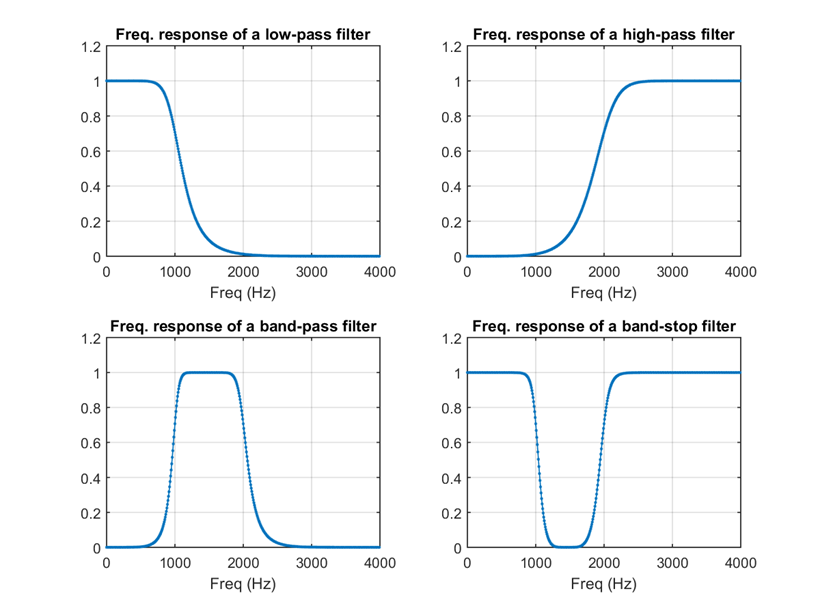
\includegraphics[width=0.75\linewidth]{Images/bandpass.png}
    \caption{Types of filters}
    \label{fig:Types of filters}
\end{figure}

\subsection{Results}
The band-pass filter effectively attenuated frequencies outside the 100 Hz to 1000 Hz range, isolating the frequencies relevant to heartbeats and lung sounds. However, low-frequency noise still permeated through, indicating that the filter did not eliminate all unwanted signals.

\begin{figure}[h]
    \centering
    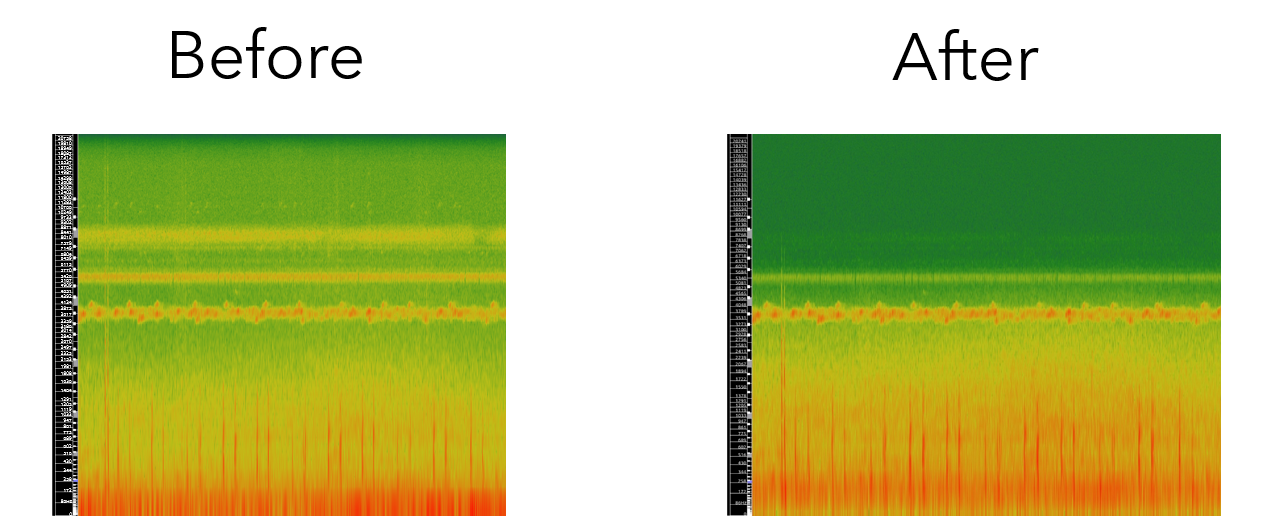
\includegraphics[width=1\linewidth]{Images/medium_obs.png}
    \caption{Mel Spectrogram before and after applying a band-pass filter to medium-level noise}
    \label{fig:enter-label}
\end{figure}

\subsection{Observations}
While the filter performed decently in removing unwanted frequencies, a significant amount of noise remained, suggesting that additional filtering techniques may be necessary. The band-pass filter can be used as the first layer of filtering, but it is not sufficient on its own to achieve the desired signal clarity.


\subsection{Conclusion}
The exploration of band-pass filters illustrated their importance in various applications in signal processing. Although effective to an extent, the need for further noise reduction strategies was highlighted.




\section{Wavelet Transform (Aryanil)} The wavelet transform is a powerful analytical tool used to study signals by decomposing them into components called wavelets. These wavelets are oscillatory functions that provide both temporal and frequency information about the signal. Unlike other transformations, such as the Fourier transform, which only gives global frequency information, the wavelet transform offers a multi-resolution perspective, enabling the analysis of the signal at different scales. The wavelet transform typically involves four key steps: defining wavelet basis functions, performing signal decomposition, conducting multi-resolution analysis, and performing signal reconstruction.

\subsection{Wavelet Basis Functions} Wavelet transforms rely on a set of basis functions known as wavelets. These wavelets are unique in that they are localized both in time and frequency, offering an adaptive resolution that adjusts to the signal's characteristics. In contrast to the Fourier transform, which decomposes a signal into sinusoidal components (sine and cosine functions), wavelets allow for better localization in both domains. This is achieved by using shorter wavelets at higher frequencies and longer wavelets at lower frequencies, providing a detailed time-frequency representation. Several types of wavelets are commonly used in signal processing, including the Haar wavelet, which is the simplest and most intuitive, and the Daubechies wavelets, which offer smoother transitions and are widely employed in practical applications.

\subsection{Decomposition} Decomposing a signal using wavelet transform involves a series of steps aimed at breaking the signal into its approximation and detail components. This process is outlined as follows:

\begin{itemize} \item \textbf{Wavelet Filters:} Initially, the signal is passed through two types of filters: a low-pass filter (often called the approximation filter) and a high-pass filter (called the detail filter). The low-pass filter captures the low-frequency components of the signal, while the high-pass filter extracts the high-frequency details. \item \textbf{Convolution:} The signal is convolved with these filters to obtain the approximation and detail coefficients. Convolution is a mathematical operation that blends the signal with the filter, allowing it to extract the relevant frequency components. \item \textbf{Downsampling:} After convolution, the number of data points is reduced by downsampling, a process where every other sample is discarded. This downsampling step ensures that the signal is represented at a lower resolution, allowing for the capture of coarser frequency bands while maintaining the essential signal features. \item \textbf{Recursive Decomposition:} The decomposition process is recursive: the approximation coefficients obtained from the first level of decomposition are passed through the same filtering and downsampling steps to achieve further levels of decomposition. This allows for analyzing the signal at multiple scales or resolutions. \end{itemize}

A visual representation of the decomposition process is shown below, where recursive filtering and subsampling occur in each iteration.

\begin{figure}[h] \centering 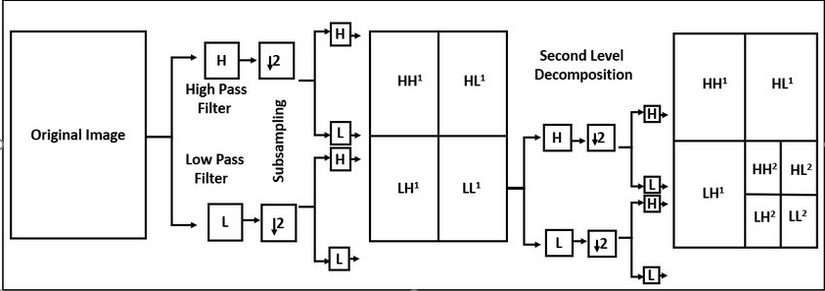
\includegraphics[width=0.8\linewidth]{Images/wavelet-decomposition.png} \caption{Two-level wavelet decomposition structure (recursive filtering and subsampling).} \label{fig:wavelet decomposition} \end{figure}

\subsection{Multi-Resolution Analysis} Multi-resolution analysis (MRA) is a key concept in wavelet transforms. It refers to the method of analyzing a signal at different levels of resolution, which is crucial for understanding both fine and coarse features of the signal. MRA enables the decomposition of a signal into multiple frequency bands, each representing different scales. This flexibility allows for a more nuanced analysis of the signal’s characteristics. For example, in biomedical signal processing, MRA can be used to separate high-frequency noise (such as electrical interference) from the low-frequency components that represent important physiological signals like heartbeats. By focusing on these different frequency bands, MRA facilitates better noise reduction and more accurate feature extraction.

In the figure below, the process of multi-resolution analysis is illustrated, showing how the signal is decomposed into components of varying frequency ranges, each representing different levels of resolution.

\begin{figure}[h] \centering 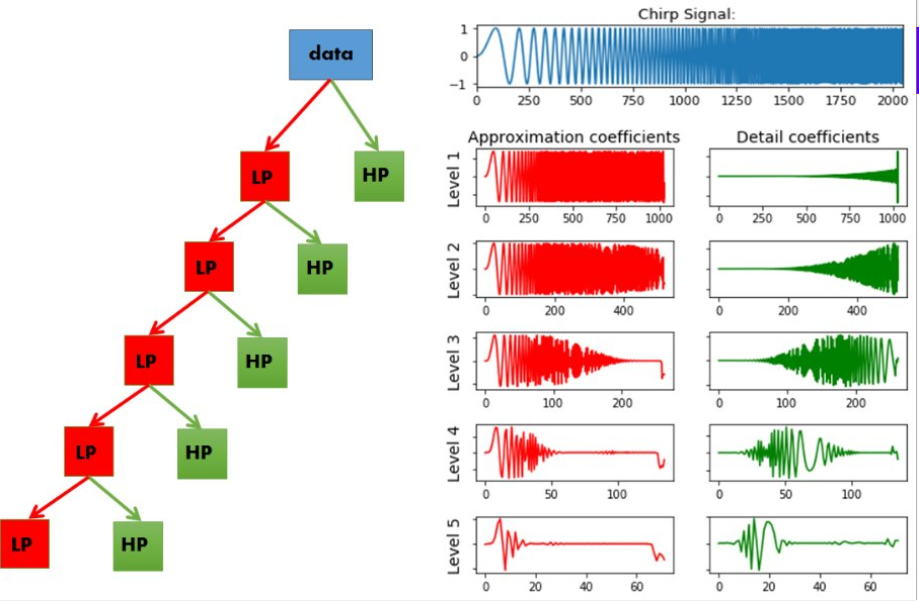
\includegraphics[width=0.8\linewidth]{Images/multi-resolution analysis.png} \caption{Multi-Resolution Analysis.} \label{fig:multiresolution analysis} \end{figure}

\subsection{Reconstruction} The goal of wavelet transform is not only to analyze the signal but also to reconstruct it accurately. Signal reconstruction is the process of combining the approximation and detail coefficients obtained from decomposition to restore the original signal. This is achieved using the inverse wavelet transform, which reverts the decomposed components back to the original signal. The reconstruction can be controlled to focus on specific frequency components by modifying the coefficients before performing the inverse transform. For instance, in applications like heartbeat detection, low-frequency components that represent the heart rate are preserved, while high-frequency noise components are filtered out, improving signal clarity and robustness.

An example of the effect of wavelet decomposition on a signal can be seen in the spectrogram comparison below. It shows the difference between a raw signal and a filtered signal after applying wavelet decomposition to reduce medium-level noise.

\begin{figure}[h] \centering 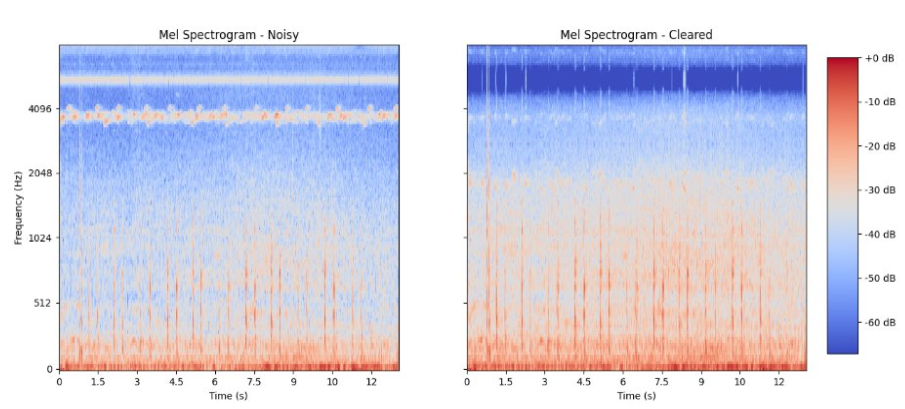
\includegraphics[width=0.8\linewidth]{Images/medium-noise mel spectrogram.png} \caption{Mel Spectrogram Before and After Wavelet Decomposition for Medium-Noise Reduction.} \label{fig:medium mel comparison} \end{figure}

% \subsection{Melodic Spectrogram Analysis}
% Melodic spectrograms were generated to visualize the effectiveness of different filtering techniques. Code was written using \texttt{librosa}, \texttt{numpy}, and \texttt{matplotlib} libraries to create spectrograms before and after filtering. Observations from the visual differences informed the development of a master pipelined algorithm.

% \subsubsection{Findings from the Graphs}
% From the spectrograms, we observed:
% \begin{itemize}
%     \item \textbf{Spectral Gating:} Extremely efficient at removing noise at the same frequency level as the heartbeat signal.
%     \item \textbf{Wavelet Transform:} Aggressively removes high-frequency noise, isolating the signal effectively.
%     \item \textbf{Bandpass Filter:} Boosts low-frequency components but fails to remove high-frequency noise.
%     \item \textbf{Noisy Environments:} Surrounding noise with overlapping frequencies makes isolation challenging.
% \end{itemize}







\section{Spectral Gating (Adithya)}
Initially, we had focused on analysing various filtering algorithms, I had researched Spectral Gating. Spectral
Gating is a noise reduction technique used in audio processing
to reduce unwanted background noise while preserving the
desired signal.
Sound in the real world, however, consists of a multitude of
such pure signals. It is difficult to, therefore, apply frequency-related operations to it. To decompose a complex sound to its
constituent frequencies, Fourier transformation is used.
Spectral Gating involves analyzing the frequency spectrogram generated by applying a Fourier transformation and
applying gates on it and obtaining the audio signal by performing the inverse Fourier transformation on the modified
spectrogram.

\subsection{Short-Time Fourier Transformation (STFT)}
The audio signal is divided into small overlapping segments
(windows). Using small windows of the audio signal for
applying a Fourier transformation is what is referred to as
the Short Time Fourrier Transformation(STFT).

\subsection{The Spectrogram}
We convert the y-axis (frequency) to a log scale and
the color dimension (amplitude) to decibels to form the
spectrogram. After obtaining the spectrogram, gates are then
applied (threshold on the amplitude) to filter out noise whose
amplitude is lower than that of the estimated threshold.

\subsection{Inverse Fourier Transformation}
After analyzing the spectrogram (whose domain is frequency) , we can apply an inverse Fourier transformation to
obtain a new modified audio signal(whose domain is time).

\begin{figure}[h]
    \centering
    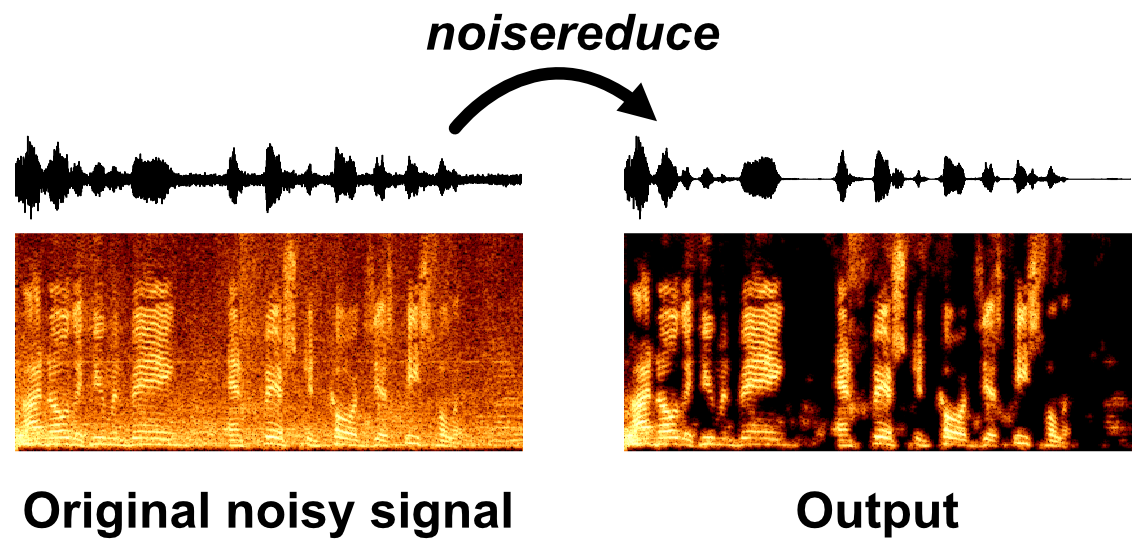
\includegraphics[width=0.8\linewidth]{Images/noisereduce.png}
    \caption{Spectral gating using `noisereduce` library in Python}
    \label{fig:spectral-gating}
\end{figure}

\subsection{Illustration}
Figure 12 shows the results of spectral gating using the `noisereduce` library.
As can be seen, the lower amplitude
sounds are filtered by the mask, which gates noise below the
frequency-varying amplitude threshold.




\section{Melodic Spectrogram Analysis (Aryanil)}
During the second week of this project, we focused on comparing melodic spectrograms generated by different filtering methods. The comparisons were made using the \texttt{librosa}, \texttt{pyplot}, and \texttt{numpy} libraries. The resulting spectrograms provide insights into the effectiveness of various signal processing techniques.



\subsection{Findings from the Graphs}
The following observations were made from the mel-spectrogram comparisons:
\begin{itemize}
    \item \textbf{Spectral Gating:} Efficient at cleaning noise at the same frequency level as the heartbeat signal.
    \item \textbf{Wavelet Transform:} Aggressively removes high-frequency noise, making it suitable for isolating heartbeat signals.
    \item \textbf{Bandpass Filter:} While it boosts low-frequency components, it fails to remove high-frequency noise.
    \item \textbf{Noisy Environments:} In loud surroundings, noise with a similar frequency to the heartbeat can drown out the signal, making it difficult to isolate.
\end{itemize}

\begin{figure}[h]
\centering
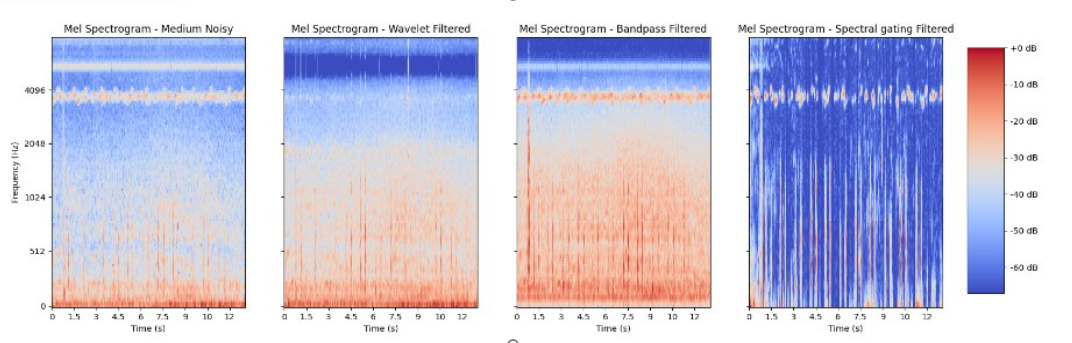
\includegraphics[width=0.8\linewidth]{Images/all methods mel spec.png}
\caption{Mel Spectrogram Before and after applying master-algorithm for Medium-Noise.}
\label{fig:mastermedium mel comparison}
\end{figure}




\section{Master Algorithm (Adithya)}
I focused on developing a master algorithm, followed by amplification of the audio signal for obtaining a filtered audio output. We had coded 3 filtering
algorithms: band-pass filters, wavelet decomposition, and spectral gating and plotted the spectrograms on the output
audio sample after applying the three filtering algorithms
individually. While we observed that the sound sample was
getting filtered to an extent, the results weren’t satisfactory.
The next step was to combine the various filtering algorithms,
i.e., pipelining the output of a filtering algorithm to the input
of another algorithm. To obtain the most optimal filtering algorithm, we tried all possible combinations of the 3 algorithms
leaving algorithms out of the filtering one by one.


\subsection{Filtering Order}
The band pass filter is applied first because concentrating on the frequency band of interest ensures that only
meaningful lung sound components are processed further. It
has been proposed that applying wavelet denoising after the
aforementioned layer of filtering followed by an adaptive filtering algorithm turns out to be effective(This is what we learnt
about in a research paper and found to be most effective). In
our case, the adaptive filtering algorithm is spectral gating.

\subsection{Amplification}
After applying the filtering algorithms in the order mentioned above, we found significant filtering of the noise, both
by inspection of the ear and by analysis of the spectrogram
plotted. However, we noticed that even the heartbeat had
become very faint as well. To fix this, we amplified the
audio by a factor of 10 by increasing the amplitude of the
audio waveform by multiplying by 10.

\subsection{Results}
After amplifying the output of the master algorithm, we had
recorded some audio samples and passed them to the master
algorithm. As shown in Fig. 17 and 18, the results after filtering
are quite satisfactory.

\begin{figure}
    \centering
    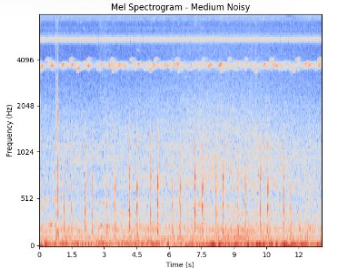
\includegraphics[width=0.8\linewidth]{Images/image.png}
    \caption{Mel-spectrogram before filtering}
    \label{fig:before-filtering}
\end{figure}

\begin{figure}
    \centering
    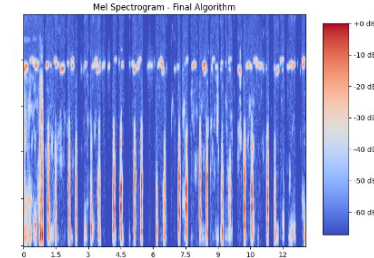
\includegraphics[width=0.8\linewidth]{Images/image2.png}
    \caption{Mel-spectrogram after filtering}
    \label{fig:after-filtering}
\end{figure}





\section{Models}



\subsection{CNN vs SVM}
We explored various ML models and implemented preliminary versions of both a 2D CNN and an SVM for our project. Each model has its own advantages, making them suitable for different scenarios. Convolutional Neural Networks (CNNs) are particularly well-suited for image data due to their ability to automatically learn hierarchical features directly from pixel data. By leveraging convolutional layers, CNNs efficiently capture spatial hierarchies and local patterns inherent in images.

On the other hand, Support Vector Machines (SVMs) can be advantageous in situations where datasets are relatively small or where computational resources are limited. SVMs excel in classification tasks with well-defined feature spaces and are often simpler to train compared to deep learning models like CNNs. However, SVMs typically require manual feature engineering, which can be time-intensive and may not capture spatial relationships as effectively as CNNs.

Given these complementary strengths, we decided to implement and evaluate both CNN and SVM models in our project to determine which performs better for our specific dataset and classification task.



\subsection{1D, 2D, and 3D CNNs}
We initially developed a preliminary code for the Image Classifier using a 2D CNN model. However, we soon encountered another challenge: most available datasets, such as the HF Lung Sound dataset, consist of .wav files, which are 1D audio waveform data. To train a 2D CNN, we needed to convert each audio file into a spectrogram, representing the audio data in a visual format suitable for image classification. Although this preprocessing step was time-intensive, it allowed us to leverage the powerful capabilities of the 2D CNN model in capturing spatial hierarchies and patterns in the spectrograms.

After carefully weighing the alternatives, including the use of a 1D CNN model designed specifically for processing 1D audio waveform data, we decided to proceed with the 2D CNN approach. By generating spectrograms for the dataset, we ensured that the model could effectively learn the intricate features present in the audio data, ultimately enabling more accurate classification results.




\section{SVM Model (Karthik)}

\subsection{Working}
\begin{itemize}
    \item \textbf{Data Input:} The SVM model receives input features derived from lung sounds, 
    such as Mel spectrograms, to represent audio patterns.
    \item \textbf{Classification:} SVM separates data into distinct classes by finding the 
    hyperplane that best divides the feature space.
    \item \textbf{Kernel Trick:} It applies a kernel function (e.g., linear, RBF) to handle 
    non-linear data more effectively.
    \item \textbf{Training and Prediction:} During training, the model learns the boundary for 
    different lung sound categories (normal, wheezing, crackles, both). In prediction, it assigns 
    a class to unseen data based on learned patterns.
\end{itemize}

\subsection{Code Explanation}
Code given as Listing 5

In this code, we load audio files from a list of file paths and extract features using the `librosa` library. These features include Mel-frequency cepstral coefficients (MFCCs), spectral centroid, spectral bandwidth, and zero-crossing rate, which are commonly used for audio classification tasks.

The function \textit{extract\_features} takes an audio file path as input and processes the audio to extract the following features:
\begin{itemize}
    \item \textbf{MFCCs}: These are the Mel-frequency cepstral coefficients, which are a representation of the short-term power spectrum of the audio.
    \item \textbf{Spectral Centroid}: This feature provides an estimate of the "center" of the spectrum, representing the brightness of the sound.
    \item \textbf{Spectral Bandwidth}: This feature measures the width of the spectrum and helps describe the texture of the sound.
    \item \textbf{Zero Crossing Rate}: This feature calculates how often the signal changes its sign, which can provide insight into the noisiness of the signal.
\end{itemize}

After extracting these features, the MFCCs are padded (if necessary) to ensure that all audio files have the same length. This is done by padding the MFCC matrix with zeros if its length is shorter than the maximum length required.

The feature vector for each audio file is then flattened into a one-dimensional array and returned as a concatenated vector, which includes both the MFCCs and the other extracted features.

The audio file paths provided in the list correspond to audio files containing different medical conditions, such as asthma, heart failure, COPD, and pneumonia. These audio files are used to train a machine-learning model to classify the conditions based on the extracted features.


\subsection{Results}
The following images illustrate the results of the SVM model on a lung sound classification task:

\begin{figure}[h!]
    \centering
    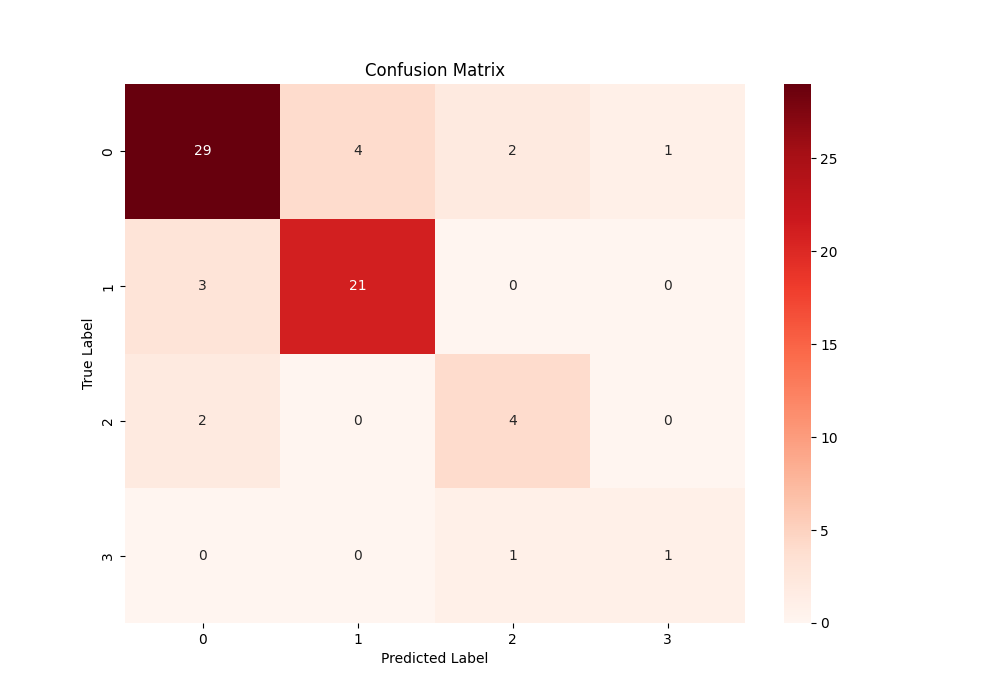
\includegraphics[width=0.4\textwidth]{Images/confusion_matrix.jpeg}
    \caption{Confusion Matrix for SVM Model}
\end{figure}

The confusion matrix shown above presents a summary of the model's performance, where each row corresponds to the true label, and each column represents the predicted label. The diagonal elements represent the number of correct predictions, while off-diagonal elements indicate misclassifications. For example, the value in the second row and the second column indicates the number of times the model correctly predicted the "wheezing" class, while the off-diagonal elements show how often the model misclassified a "wheezing" sound as another class.

\begin{figure}[h!]
    \centering
    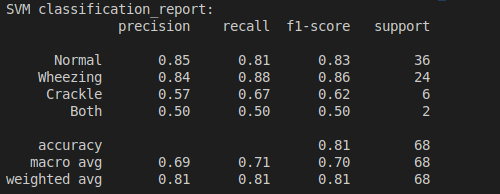
\includegraphics[width=0.4\textwidth]{Images/SVM.png}
    \caption{SVM Classification Report}
\end{figure}

The classification report provides additional insight into the model's performance, showing metrics such as precision, recall, and F1-score for each class. Precision measures the accuracy of positive predictions (e.g., how many of the predicted "wheezing" instances were actually wheezing), recall indicates how many actual instances of a class were correctly identified, and the F1-score is the harmonic mean of precision and recall. This report helps to evaluate the overall effectiveness of the model, highlighting areas where it performs well (e.g., classifying "normal" and "wheezing" sounds) and areas that may need improvement (e.g., classifying "both" sounds).

In summary, the SVM model shows strong performance in classifying lung sounds into different categories, but further tuning, data preprocessing, and additional features (such as spectral features) may be required to improve accuracy and handle more complex audio conditions effectively.







\section{Implementation of 2D CNN model (Adithya)}{
We implemented the CNN model by splitting it into two parts, one part was for training the model on a dataset and the other was for predicting the result based on the input. In this section, we shall explore the implementation of this model and compare its accuracy with preexisting models.

\subsection{Dataset}{
We trained our model on a dataset of lung sounds recorded from the chest wall using an electronic stethoscope. This dataset contains annotated audio files (separate combined annotation files) of lung sounds as recorded from various vantage points of the chest wall. The annotation includes the sound type (Inspiratory: I, Experiatory: E, Wheezes: W, Crackles: C, Normal: N).
}
\subsection{Training the CNN model}
One part of our code trains the model for classifying lung sound audio files into different categories, such as "Normal," "Wheezing," "Crackle," and "Both" (for combined wheezing and crackle sounds). The code has been mentioned below, we shall offer a brief overview here. The audio preprocessing is done by extracting the Mel spectrograms from the raw audio data. The dataset is loaded Each audio file is processed into a Mel-spectrogram, and its corresponding label (Normal, Wheezing, Crackle, or Both) is assigned based on the file's name.
Our CNN model is defined using Keras' Sequential() API. The model consists of three convolutional layers, each followed by max-pooling, a flattening layer, a dense layer with dropout for regularization, and a final softmax output layer for classification.
Finally, The model is compiled with the Adam optimizer and sparse categorical cross-entropy loss and is trained for 10 epochs using the training data, while validating on the validation data.
After training, the model is saved as a .h5 file for future use.

\subsection{Using the CNN model for prediction}
The other part of the code is used for predicting the class of a lung sound audio file. As before, a brief overview shall be presented here.
The code takes the file path of an audio file as input, loads the pre-trained CNN model, and processes the audio file to extract and pad its Mel-spectrogram.
The spectrogram is then reshaped to fit the model's input requirements (adding the batch and channel dimensions) and passed through the CNN for classification.
The predicted class is determined by finding the class with the highest prediction score, and the corresponding label is retrieved from reverse class mapping.
The code finally returns the predicted class label (e.g., "Normal," "Wheezing," "Coughing," or "Both") along with the model's confidence score for the prediction.


\subsection{Evaluation Method and Criteria}
To evaluate the performance of our model, we generated a classification report as well as a confusion matrix at the time of training our model.
The performance criteria were selected as accuracy, recall, support, precision, and F-score.
Accuracy measures the overall correctness of the model. It is calculated as the ratio of correct predictions to the total number of predictions.

\[
\text{Accuracy} = \frac{TP + TN}{TP + TN + FP + FN}
\]

Where:
\begin{itemize}
    \item \( TP \) = True Positives (correctly predicted positive cases)
    \item \( TN \) = True Negatives (correctly predicted negative cases)
    \item \( FP \) = False Positives (incorrectly predicted positive cases)
    \item \( FN \) = False Negatives (incorrectly predicted negative cases)
\end{itemize}

Recall(Sensitivity or True Positive Rate) measures the proportion of actual positive cases that are correctly identified by the model. It is defined as:

\[
\text{Recall} = \frac{TP}{TP + FN}
\]

Where:
\begin{itemize}
    \item \( TP \) = True Positives
    \item \( FN \) = False Negatives
\end{itemize}

Precision measures the proportion of predicted positive cases that are actually positive. It is given by:

\[
\text{Precision} = \frac{TP}{TP + FP}
\]

Where:
\begin{itemize}
    \item \( TP \) = True Positives
    \item \( FP \) = False Positives
\end{itemize}

The F1-score is the harmonic mean of precision and recall. It balances the two metrics and is useful when the classes are imbalanced. The formula is:

\[
\text{F1-Score} = 2 \times \frac{\text{Precision} \times \text{Recall}}{\text{Precision} + \text{Recall}}
\]

Support refers to the number of true instances of each class in the dataset. It is the count of occurrences of each class and is used to calculate other metrics:

\[
\text{Support} = \text{Number of true instances of a class}
\]


\begin{figure}
    \centering
    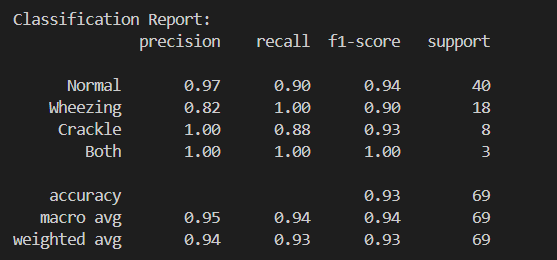
\includegraphics[width=0.8\linewidth]{Images/Screenshot 2024-11-12 133318.png}
    \caption{Classification report of 2D CNN model}
    \label{fig:spectral-gating}
\end{figure}

\begin{figure}
    \centering
    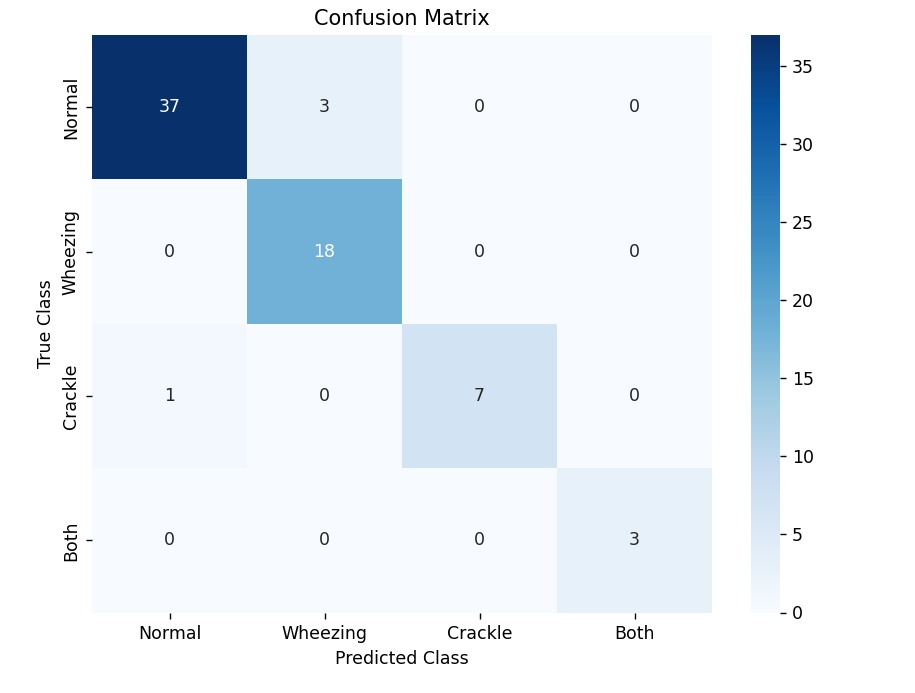
\includegraphics[width=0.8\linewidth]{Images/WhatsApp Image 2024-12-03 at 11.10.05 PM.jpeg}
    \caption{Confusion Matrix of 2D CNN model}
    \label{fig:spectral-gating}
\end{figure}

\subsection{Comparision with existing models}

In this study, our model achieved an accuracy of \textbf{93\%} using a CNN model with Mel Spectrograms, which is competitive with existing methods in the literature. Table~\ref{tab:accuracy_comparison} summarizes the comparison with other studies. Notably, A. S. Edakkadan and A. Srivastava(2023) achieved an accuracy of \textbf{80.55\%} using a CNN model with Mel Spectrograms, while  F. Demir, A. M. Ismael, and A. Sengur(2020) reported an accuracy of \textbf{71.15\%} with CNN Model with Parallel Pooling Structure. These results highlight the effectiveness of our method in [specific context, e.g., handling noisy data or small datasets]. Also, F. Demir, A. Sengur, and V. Bajaj (2020) achieved an accuracy of \textbf{65.50\%} using Deep Feature with VGG-16 CNN model and SVM classifier.

\begin{table}[h!]
\centering
\begin{tabular}{|c|c|c|}
\hline
\textbf{Study}                      & \textbf{Accuracy (\%)}            \\ \hline
Our Model                      & 93                                     \\ \hline
A. S. Edakkadan and A. Srivastava(2023)     &  80.55                  \\ \hline
F. Demir, A. M. Ismael and A. Sengur(2020)             & 71.15         \\ \hline
F. Demir, A. Sengur, and V. Bajaj, (2020)     &  65.50                  \\ \hline
 
\end{tabular}
\caption{Comparison of our model's accuracy with other studies.}
\label{tab:accuracy_comparison}
\end{table}









\section{Website (Aryanil, Anurag)}
The website was designed to provide a user-friendly interface for real-time lung sound analysis.

\begin{figure}[h]
    \centering
    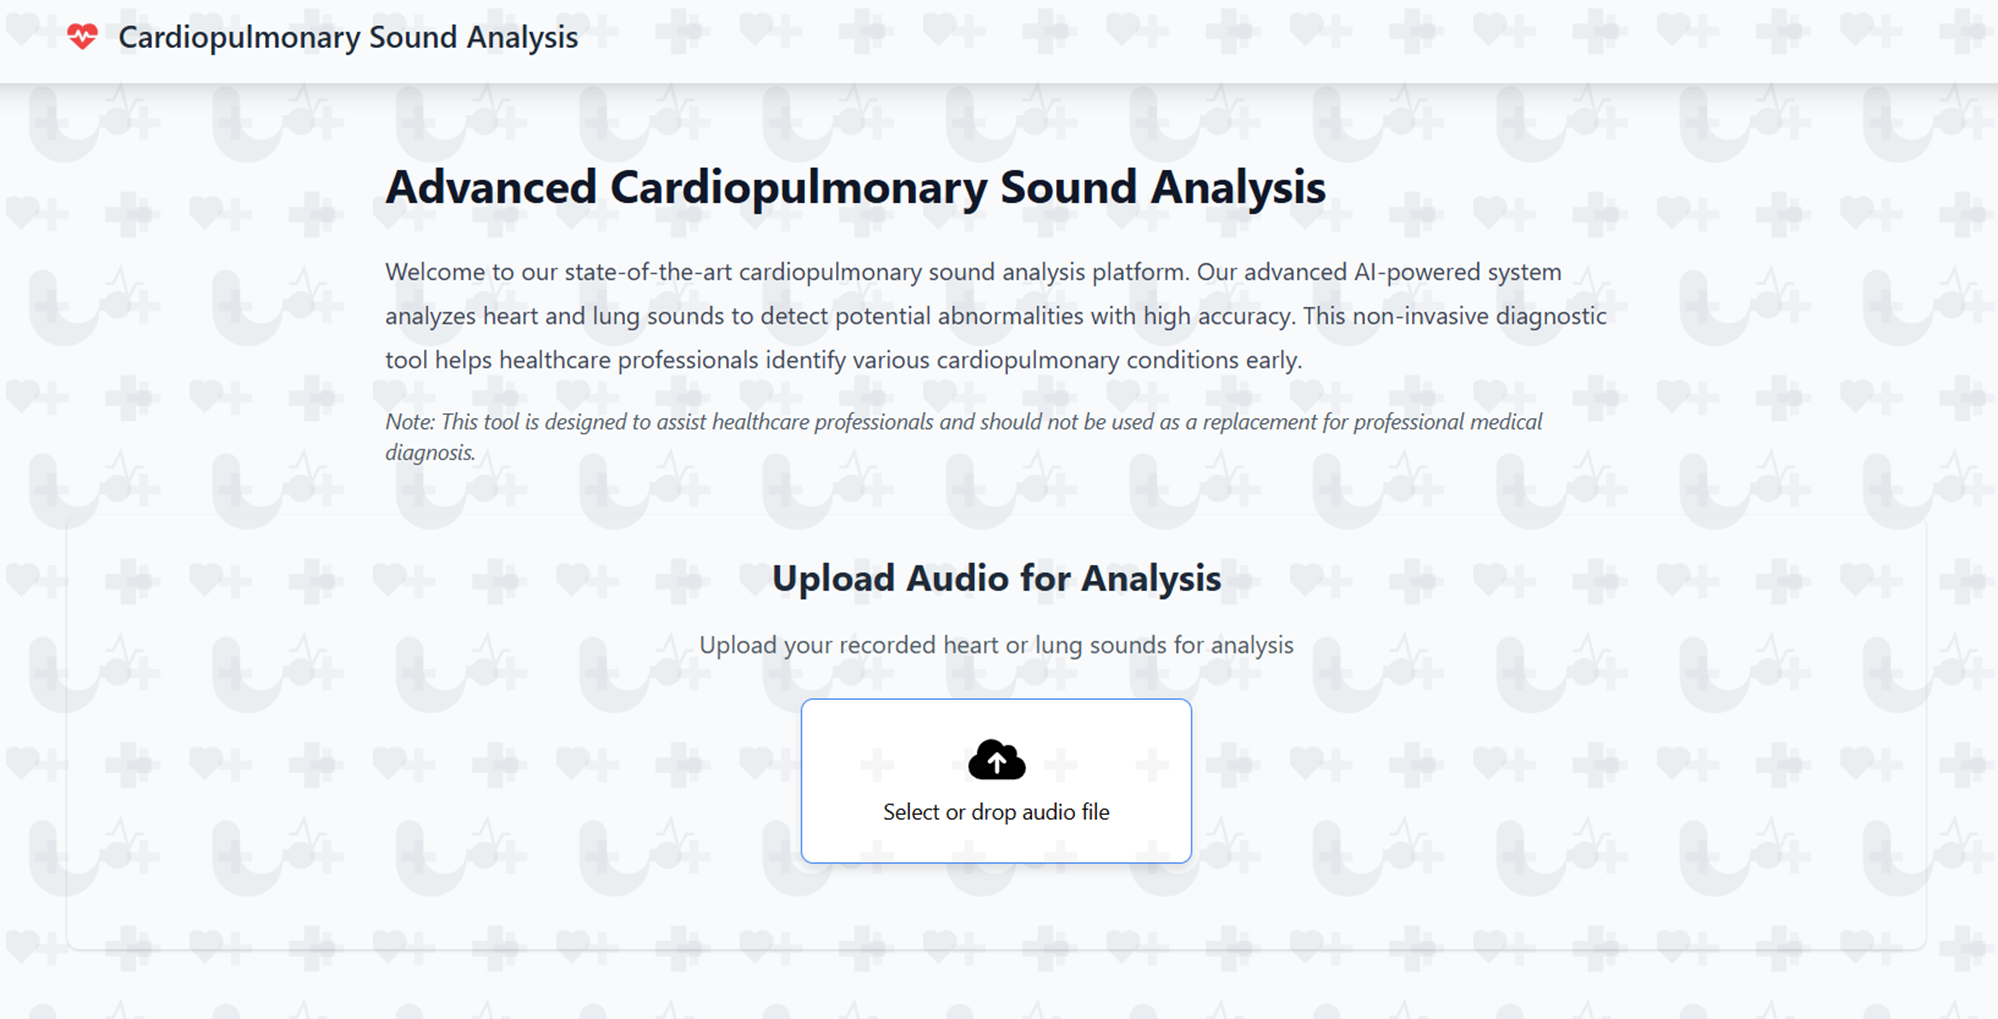
\includegraphics[width=1\linewidth]{Images/website.png}
    \caption{Website UI}
    \label{fig:enter-label}
\end{figure}

\subsection{Website Features}
The lung sound detection system is designed with an intuitive and user-friendly web interface that simplifies the process of audio analysis for medical practitioners and researchers. Below are the detailed features of the website:

\subsubsection{Drag-and-Drop Functionality}
The website allows users to easily upload audio files through a drag-and-drop interface. This feature ensures a seamless and efficient workflow, eliminating the need for complex navigation or manual file selection.

\subsubsection{Automated Audio Analysis Pipeline}
Once an audio file is uploaded, it passes through a robust analysis pipeline. Key steps in this pipeline include:
\begin{itemize}
    \item \textbf{Preprocessing:} Noise reduction using wavelet decomposition and spectral filtering.
    \item \textbf{Feature Extraction:} Generation of spectrograms and extraction of key acoustic features.
    \item \textbf{Classification:} Using machine learning models to identify potential lung conditions.
\end{itemize}

\subsubsection{Disease Confidence Scores}
The system provides detailed confidence scores for identified diseases. These scores represent the model's certainty, helping users assess the reliability of the diagnosis.

\subsubsection{Real-Time Visualization}
Analysis results are displayed in an easy-to-understand format, including:
\begin{itemize}
    \item Spectrograms of the uploaded audio before and after filtering.
    \item Identified disease labels with their respective confidence levels.
\end{itemize}

\subsubsection{Responsive and Accessible Design}
The website is designed to be responsive, ensuring optimal performance on devices of various screen sizes. Accessibility features include clear navigation, keyboard-friendly interactions, and support for assistive technologies.


\subsection{Backend}
	We used the \texttt{Flask} module in Python to implement the backend of the application. The uploaded file is given as input to a saved model, which predicts the class label for the given sound.
	
	Custom-written modules written for SVM and CNN were used to use the saved model to output a prediction along with a confidence score. These results are then shown on the website.
	
	\begin{figure}[h]
		\centering
		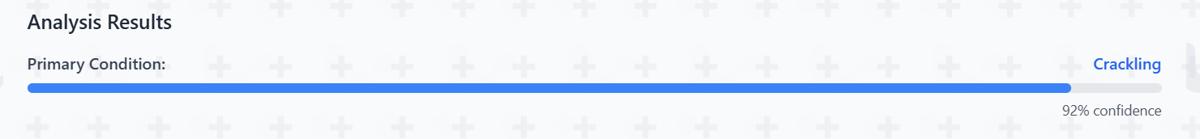
\includegraphics[width=1\linewidth]{Images/website_output.png}
		\caption{Label and confidence score output}
		\label{fig:enter-label}
	\end{figure}







\section*{Acknowledgment}
The author thanks Prof. Abishek, Srikar, and Santoshini for their guidance and resources. Special thanks to the open-source community for libraries like `librosa`, `matplotlib`, `noisereduce`, and `numpy`.

\begin{thebibliography}{1}

\bibitem{ref1}
Noisereduce GitHub: \url{https://github.com/timsainb/noisereduce}

\bibitem{ref2}
Dataset for training the models: 
\url{https://data.mendeley.com/datasets/jwyy9np4gv/3}

\bibitem{ref3}
F. Demir, A. M. Ismael and A. Sengur, "Classification of Lung Sounds With CNN Model Using Parallel Pooling Structure," in IEEE Access, vol. 8, pp. 105376-105383, 2020, doi: 10.1109/ACCESS.2020.3000111.

\bibitem{ref4}
F. Demir, A. Sengur, and V. Bajaj, ‘‘Convolutional neural networks based
efficient approach for classification of lung diseases,’’ Health Inf. Sci. Syst.,
vol. 8, no. 1, pp. 1–8, Dec. 2020.

\bibitem{ref5}
Adithya Sunil Edakkadan, Abhishek Srivastava, \textit{Deep Learning Based Portable Respiratory Sound Classification System}, IEEE, 2023.



\end{thebibliography}










\section*{Reference Codes}


\textbf{Note:} These and other codes can all be found on GitHub at \url{https://github.com/AryanilPanja/lung_sound_recorder}
\\


\begin{lstlisting}[style=mypython, caption={Code for Generating a Mel-Spectrogram}, label={lst:mel-spectrogram}]
import librosa
import librosa.display
import matplotlib.pyplot as plt
import numpy as np

def plot_mel_spectrogram(ax, data, sr, title, fmax=8000):

    S = librosa.feature.melspectrogram(y=data, sr=sr, n_mels=128, fmax=fmax)
    S_dB = librosa.power_to_db(S, ref=np.max)
    
    img = librosa.display.specshow(S_dB, sr=sr, x_axis='time', y_axis='mel', fmax=fmax, cmap='coolwarm', ax=ax)
    ax.set_title(title)
    ax.set_xlabel('Time (s)')
    ax.set_ylabel('Frequency (Hz)')
    ax.label_outer()

    return img

# Load audio files accordingly
file_path1 = './../steth_record/computer.wav'  
file_path2 = './../filtered_algo/heartbeat_tube_filtered.wav'  

data1, sr1 = librosa.load(file_path1, sr=None)
data2, sr2 = librosa.load(file_path2, sr=None)

# Create a figure with four subplots
fig, (ax1, ax2) = plt.subplots(1, 2, figsize=(17, 6), sharex=True, sharey=True)

# Plot Mel spectrograms for all four audio files
img1 = plot_mel_spectrogram(ax1, data1, sr1, 'Mel Spectrogram -  Computer Heartbeat Soft-noisy ')
img2 = plot_mel_spectrogram(ax2, data2, sr2, 'Mel Spectrogram - Final Algorithm clean')

plt.subplots_adjust(right=0.85)

cbar_ax = fig.add_axes([0.87, 0.15, 0.03, 0.7])  # [left, bottom, width, height]
fig.colorbar(img1, cax=cbar_ax, format='%+2.0f dB')

plt.savefig('desired_name.png')

\end{lstlisting}


\begin{lstlisting}[style=mypython, caption={Python code for Butterworth band-pass filter}]
from scipy.signal import butter, lfilter

def butter_bandpass(lowcut, highcut, fs, order=5):
nyq = 0.5 * fs
low = lowcut / nyq
high = highcut / nyq
b, a = butter(order, [low, high], btype='band')
return b, a


def butter_bandpass_filter(data, lowcut, highcut, fs, order=5):
b, a = butter_bandpass(lowcut, highcut, fs, order=order)
y = lfilter(b, a, data)
return y

import numpy as np
import librosa
import soundfile as sf

# Sample rate and desired cutoff frequencies (in Hz).
fs = 5000.0
lowcut = 10.0
highcut = 400.0

noise, samplerate = librosa.load('loudnoise.wav', sr=None)

y = butter_bandpass_filter(noise, lowcut, highcut, fs, order=6)
print(len(y))
print(y)

sf.write('loud.wav', y, samplerate=samplerate)
\end{lstlisting}



\begin{lstlisting}[style=mypython, caption={Code for cleaning the sound using wavelet transform}, label={lst:mel-spectrogram}]
import librosa
import pywt
import numpy as np
from scipy.io.wavfile import write

# Load audio file
file_path = './../orig_audio/loudnoise.wav'  
data, fs = librosa.load(file_path, sr=None)

def wavelet_denoise(data, wavelet='db4', level=3):
    coeff = pywt.wavedec(data, wavelet, mode='per', level=level)

    sigma = np.median(np.abs(coeff[-level])) / 0.6745
    uthresh = sigma * np.sqrt(2 * np.log(len(data)))

    denoised_coeff = [coeff[0]]  # Keep the approximation coefficients (first element) unmodified
    denoised_coeff += [pywt.threshold(c, value=uthresh, mode='soft') for c in coeff[1:]]

    denoised_signal = pywt.waverec(denoised_coeff, wavelet, mode='per')

    if len(denoised_signal) > len(data):
        denoised_signal = denoised_signal[:len(data)]
    elif len(denoised_signal) < len(data):
        padding = np.zeros(len(data) - len(denoised_signal))
        denoised_signal = np.concatenate([denoised_signal, padding])
    
    return denoised_signal

denoised_data = wavelet_denoise(data, wavelet='db4', level=3)

output_path = 'denoised_loud_heart_sound.wav'
write(output_path, fs, (denoised_data * 32767).astype(np.int16))  # Rescale to 16-bit PCM format
    
\end{lstlisting}






\begin{lstlisting}[style=mypython, caption={Master Algorithm with Amplification}, label={lst:master-algorithm}]
import numpy as np
from scipy.signal import butter, lfilter, spectrogram
import pywt
import librosa

# Bandpass Filter
def butter_bandpass_filter(data, lowcut, highcut, fs, order=6):
    nyq = 0.5 * fs
    low = lowcut / nyq
    high = highcut / nyq
    b, a = butter(order, [low, high], btype='band')
    return lfilter(b, a, data)

# Wavelet Denoising
def wavelet_denoise(data, wavelet='db4', level=3):
    coeff = pywt.wavedec(data, wavelet, mode='per', level=level)
    sigma = np.median(np.abs(coeff[-level])) / 0.6745
    uthresh = sigma * np.sqrt(2 * np.log(len(data)))
    denoised_coeff = [coeff[0]] + [pywt.threshold(c, value=uthresh, mode='soft') for c in coeff[1:]]
    return pywt.waverec(denoised_coeff, wavelet, mode='per')

# Frequency-Aware Noise Suppression
def frequency_aware_suppression(data, sr, lung_band=(200, 1000), heart_band=(20, 200)):
    stft = librosa.stft(data)
    magnitude, phase = librosa.magphase(stft)
    frequencies = librosa.fft_frequencies(sr=sr)

    # Weight frequency bands
    weights = np.ones_like(frequencies)
    weights[(frequencies >= heart_band[0]) & (frequencies <= heart_band[1])] *= 2.0  # Suppress heart sounds
    weights[(frequencies >= lung_band[0]) & (frequencies <= lung_band[1])] *= 0.5  # Preserve lung sounds

    # Apply weights to magnitude
    magnitude = magnitude * weights[:, np.newaxis]
    return librosa.istft(magnitude * phase)

# Main Filtering Pipeline
def lung_sound_filtering(data, sr):
    filtered = butter_bandpass_filter(data, lowcut=200, highcut=1000, fs=sr)
    denoised = wavelet_denoise(filtered, wavelet='db4', level=3)
    enhanced = frequency_aware_suppression(denoised, sr)
    return np.clip(enhanced * 10, -1.0, 1.0)  # Amplify and normalize

# Example Usage
filtered_data = lung_sound_filtering(data, sr)

# Save the filtered audio
import soundfile as sf
sf.write("lung_sound_filtered.wav", filtered_data, sr)

\end{lstlisting}











'

\begin{lstlisting}[style=mypython, caption={Python code for SVM Model}]
import librosa
import numpy as np
from sklearn.svm import SVC
from sklearn.model_selection import train_test_split
from sklearn.metrics import classification_report
from sklearn.preprocessing import LabelEncoder

from sklearn.metrics import classification_report, confusion_matrix
import seaborn as sns
import matplotlib.pyplot as plt


# Function to extract MFCC features from an audio file
def extract_features(audio_file, max_length):
    y, sr = librosa.load(audio_file, sr=None)
    mfccs = librosa.feature.mfcc(y=y, sr=sr, n_mfcc=13)
    spectral_centroid = np.mean(librosa.feature.spectral_centroid(y=y, sr=sr))
    spectral_bandwidth = np.mean(librosa.feature.spectral_bandwidth(y=y, sr=sr))
    zero_crossing_rate = np.mean(librosa.feature.zero_crossing_rate(y=y))
    
    if mfccs.shape[1] < max_length:
        pad_width = max_length - mfccs.shape[1]
        mfccs = np.pad(mfccs, ((0, 0), (0, pad_width)), mode='constant')
    else:
        mfccs = mfccs[:, :max_length]
        
    return np.concatenate((mfccs.flatten(), [spectral_centroid, spectral_bandwidth, zero_crossing_rate]))


# Corrected file paths
file_paths = [
    # File names present here
]

labels = [ # labels corresponding to the approriate file names ]

features = []
for file in file_paths:
    mfcc_features = extract_features(file, 7500)
    features.append(mfcc_features)

# Convert to numpy array for sklearn
X = np.array(features)
y = np.array(labels)

label_encoder = LabelEncoder()
y_encoded = label_encoder.fit_transform(y)

# Split the dataset into training and testing sets
X_train, X_test, y_train, y_test = train_test_split(X, y_encoded, test_size=0.2, random_state=42)

# Initialize the SVC model
model = SVC(kernel='linear')

# Train the model
model.fit(X_train, y_train)

# Make predictions
y_pred = model.predict(X_test)
y_pred_transformed = label_encoder.inverse_transform(y_pred)
y_test_transformed = label_encoder.inverse_transform(y_test)

class_mapping = {
    'Normal': 0,
    'Wheezing': 1,
    'Crackle': 2,
    'Both': 3
}
unique_classes = np.unique(y_test)
target_names = [list(class_mapping.keys())[i] for i in unique_classes]

# Evaluate the model
print("SVM classification_report:")
print(classification_report(y_test_transformed, y_pred_transformed, target_names=target_names))

# Confusion matrix
conf_matrix = confusion_matrix(y_test, y_pred)
plt.figure(figsize=(10, 7))
sns.heatmap(conf_matrix, annot=True, fmt='d', cmap='Reds', xticklabels=label_encoder.classes_, yticklabels=label_encoder.classes_)
plt.xlabel("Predicted Label")
plt.ylabel("True Label")
plt.title("Confusion Matrix")

# Save the confusion matrix as an image
plt.savefig("confusion_matrix.png")
print("Confusion matrix saved as 'confusion_matrix.png'")
\end{lstlisting}





\begin{lstlisting}[style=mypython, caption={Code for training the CNN Model}, label={lst:cnn-model_train}]

import os
import numpy as np
import librosa
from sklearn.model_selection import train_test_split
from tensorflow.keras import layers, models
from sklearn.metrics import confusion_matrix, classification_report
import seaborn as sns
import matplotlib.pyplot as plt

def extract_mel_spectrogram(file_path):
    y, sr = librosa.load(file_path, sr=None)
    mel_spectrogram = librosa.feature.melspectrogram(y=y, sr=sr, n_mels=128)
    log_mel_spectrogram = librosa.power_to_db(mel_spectrogram)
    return log_mel_spectrogram

def pad_spectrogram(mel_spectrogram, max_len):
    if mel_spectrogram.shape[1] < max_len:
        pad_width = max_len - mel_spectrogram.shape[1]
        mel_spectrogram = np.pad(mel_spectrogram, ((0, 0), (0, pad_width)), mode='constant')
    else:
        mel_spectrogram = mel_spectrogram[:, :max_len]
    return mel_spectrogram

# Directory containing your audio files
data_dir = './dataset/Audio_Files' 
labels = []
mel_spectrograms = []

class_mapping = {
    'Normal': 0,
    'Wheezing': 1,
    'Crackle': 2,
    'Both': 3
}

count1 = 0
count2 = 0
count3 = 0
count4 = 0


# Load data
for file in os.listdir(data_dir):
    if file.endswith('.wav'):
        file_path = os.path.join(data_dir, file)
        mel_spec = extract_mel_spectrogram(file_path)
        mel_spectrograms.append(mel_spec)
        
        # Determine the label based on the file name
        
        label = "Normal"
        if "W," in file_path or ' W' in file_path:
            if "C," in file_path or 'C ' in file_path:
                label = "Both"
                count4 = count4 + 1
                print(file_path)
                
            else:
                label = "Wheezing"
                count3 = count3 + 1
        elif "C," in file_path or 'C ' in file_path:
            label = "Crackle"
            count2 = count2 + 1
        else:
            count1 = count1 + 1
        labels.append(class_mapping[label])



# Prepare data for training
max_len = 250
mel_spectrograms_padded = [pad_spectrogram(mel_spec, max_len) for mel_spec in mel_spectrograms]
X_padded = np.array(mel_spectrograms_padded)[..., np.newaxis]  # Add channel dimension
y = np.array(labels)

# Split into training and validation sets
X_train, X_val, y_train, y_val = train_test_split(X_padded, y, test_size=0.2, random_state=32)

# Create CNN model
def create_cnn_model(input_shape, num_classes):
    model = models.Sequential([
        layers.Conv2D(32, (3, 3), activation='relu', input_shape=input_shape),
        layers.MaxPooling2D(pool_size=(2, 2)),
        layers.Conv2D(64, (3, 3), activation='relu'),
        layers.MaxPooling2D(pool_size=(2, 2)),
        layers.Conv2D(128, (3, 3), activation='relu'),
        layers.MaxPooling2D(pool_size=(2, 2)),
        layers.Flatten(),
        layers.Dense(128, activation='relu'),
        layers.Dropout(0.5),
        layers.Dense(num_classes, activation='softmax')
    ])
    return model

input_shape = (X_padded.shape[1], X_padded.shape[2], 1)
num_classes = len(class_mapping)

model = create_cnn_model(input_shape, num_classes)
model.compile(optimizer='adam', loss='sparse_categorical_crossentropy', metrics=['accuracy'])

# Train the model
model.fit(X_train, y_train, validation_data=(X_val, y_val), epochs=10, batch_size=32)

# Evaluate the model
loss, accuracy = model.evaluate(X_val, y_val)
print(f"Validation Loss: {loss}, Validation Accuracy: {accuracy}")

# Predictions
y_pred = model.predict(X_val)
y_pred_classes = np.argmax(y_pred, axis=1)

# Check unique classes in validation set
unique_classes = np.unique(y_val)
target_names = [list(class_mapping.keys())[i] for i in unique_classes]
print("Unique classes in y_val:", np.unique(y_val))

# Classification Report
print("\nClassification Report:")
print(classification_report(y_val, y_pred_classes, labels=unique_classes, target_names=target_names))

# Confusion Matrix
conf_matrix = confusion_matrix(y_val, y_pred_classes, labels=unique_classes)
plt.figure(figsize=(8, 6))
sns.heatmap(conf_matrix, annot=True, fmt='d', cmap='Blues', xticklabels=target_names, yticklabels=target_names)
plt.title('Confusion Matrix')
plt.xlabel('Predicted Class')
plt.ylabel('True Class')
plt.show()

print(count1)
print(count2)
print(count3)
print(count4)


# Save the trained model
model.save('lung_sound_cnn_model.h5')
print("Model saved as lung_sound_cnn_model.h5")


\end{lstlisting}

\begin{lstlisting}[style=mypython, caption={Code for using the CNN model to make predictions}, label={lst:cnn-model_predict}]
import numpy as np
import librosa
from tensorflow.python.keras.models import load_model

def extract_mel_spectrogram(file_path):
    y, sr = librosa.load(file_path, sr=None)
    mel_spectrogram = librosa.feature.melspectrogram(y=y, sr=sr, n_mels=128)
    log_mel_spectrogram = librosa.power_to_db(mel_spectrogram)
    return log_mel_spectrogram

def pad_spectrogram(mel_spectrogram, max_len):
    if mel_spectrogram.shape[1] < max_len:
        pad_width = max_len - mel_spectrogram.shape[1]
        mel_spectrogram = np.pad(mel_spectrogram, ((0, 0), (0, pad_width)), mode='constant')
    else:
        mel_spectrogram = mel_spectrogram[:, :max_len]
    return mel_spectrogram

class_mapping = {
    'Normal': 0,
    'Wheezing': 1,
    'Coughing': 2,
    'Both': 3
}
reverse_class_mapping = {v: k for k, v in class_mapping.items()}

def predict_class_cnn(file_path, max_len=250):

    # Load the saved model
    model = load_model('../lung_sound_cnn_model.h5')

    mel_spec = extract_mel_spectrogram(file_path)
    padded_mel_spec = pad_spectrogram(mel_spec, max_len)
    padded_mel_spec = np.expand_dims(padded_mel_spec, axis=-1)  # Add channel dimension
    padded_mel_spec = np.expand_dims(padded_mel_spec, axis=0)   # Add batch dimension
    predictions = model.predict(padded_mel_spec)
    predicted_class_index = np.argmax(predictions, axis=1)[0]
    predicted_class = reverse_class_mapping[predicted_class_index]
    confidence = predictions[predicted_class_index]
    return [predicted_class, confidence]

""" # Example usage:
new_audio_file_path = './dataset/Audio_files2/asthma/BP1_Asthma,I E W,P L L,70,M.wav'
predicted_label = predict_class(new_audio_file_path, model)

print(f"The predicted label for the audio file is: {predicted_label}") """

\end{lstlisting}



\end{document}


